\chapter{Environnement du projet}
\section*{Introduction}

Dans ce chapitre nous allons présenter l'environnement matériel du projet, ainsi que les outils logiciels utilisés à savoir Rational DOORS, CANoe, ASAP2 et EXAM pour la gestion des exigences, lecture des fichiers de mesures de signaux et enfin créer et simuler les scripts de tests sur le Hardware-in-Loop (HiL).

\section{Environnement matériel : Harware in Loop}

Après avoir fait une petite introduction des différentes fonctions du système AWC, on passe à l’environnement où on doit exécuter nos scripts de tests qui le HiL.

La simulation HiL Hardware in Loop est une méthode de simulation caractérisée par l’association de véritables composants, connectés à une partie temps réel simulée. Souvent, les systèmes de contrôles matériel et logiciel sont identiques à ceux retenus pour la production finale. 

Le processus à contrôler comme les actionneurs et les capteurs, peut être composé soit d’éléments simulés, soit d’éléments réels. En général, un mixe des deux est réalisé. Habituellement, les actionneurs sont réels cela s’explique par le fait que les actionneurs sont difficilement modélisables.

Dans le domaine de l’automobile, le HiL met à notre disposition un véhicule virtuel afin d’exécuter toutes sortes de tests et vérification. Malheureusement, dans notre cas le HiL se trouvait dans l’Allemagne et développer par dSPACE.

\begin{figure}[H]
 \centering
 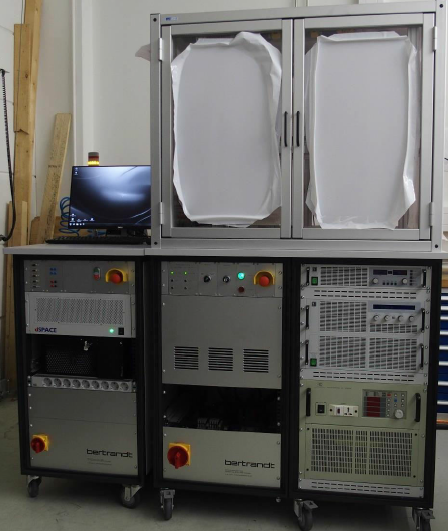
\includegraphics[scale=0.8]{images/hil}
 \caption{Station de test HiL}
\end{figure}

Sur l’image ci-dessus, on peut distinguer deux parties dans le HiL : la partie LV-Rack (Low Voltage Rack) qui est à gauche et la partie HV-Rack (High Voltage Rack) qui est à droite.

\subsection{Partie LV-Rack}

\textbf{LV-Rack} contient la partie avec les composants nécessitant une tension faible.

\begin{figure}[H]
 \centering
 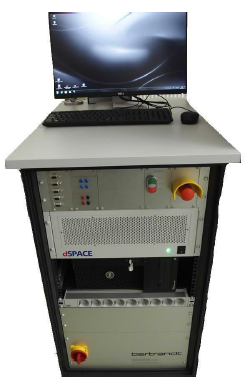
\includegraphics[scale=1]{images/lv_rack}
 \caption{Partie LV-Rack}
\end{figure}

\noindent Cette partie contient : 

\begin{itemize}
	\item Interrupteur
	\item Bande de puissance
	\item Interrupteur principal pour dSPACE
	\item Bouton d’urgence
	\item Bouton marche / arrêt pour le circuit principal
	\item Les différentes connexion CAN au système
	\item Une interface pour l’autre partie HV-Rack
	\item Capteur de champ magnétique
	\item Capteur de température infrarouge
\end{itemize}

\subsection{HV-Rack}

\textbf{HV-Rack} contient les composants nécessitant une haute tension ainsi que les composants responsables du stockage des mesures de l’ORU et le Wayside.

\begin{figure}[H]
 \centering
 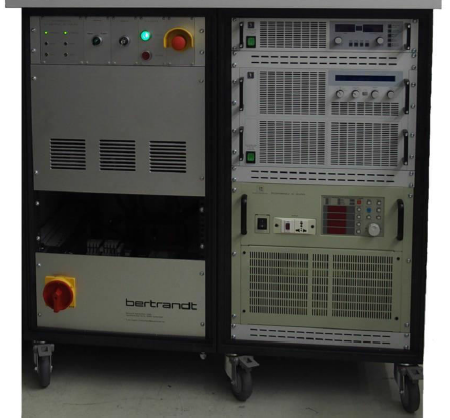
\includegraphics[scale=1]{images/hv_rack}
 \caption{Partie HV-Rack}
\end{figure}

\noindent Cette partie contient :

\begin{itemize}
	\item Interrupteur principale pour le HV-Rack
	\item Compteur de puissance
	\item Bouton d’urgence
	\item Commande de verrouillage de porte
	\item Bouton d’urgence à clé
	\item Adaptateur secteur DC HV
	\item Adaptateur secteur AC
	\item Prise d’alimentation pour l’ORU
	\item Interface pour LV-Rack
\end{itemize}

\subsection{Banc de test}

Avant, dans cette partie, on avait le Wayside qui était sur le sol avec l’ORU qu’on pouvait déplacer et tourner au-dessus du Wayside manuellement avec un levier. Mais après on a intégré un robot appelé Kuka qui s’occupe de ces opérations.

\begin{figure}[H]
 \centering
 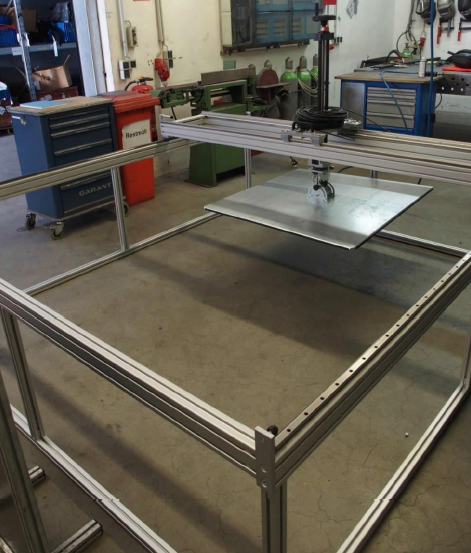
\includegraphics[scale=0.8]{images/banc_test}
 \caption{Banc de test}
\end{figure}

Le placement du Wayside est mené par un opérateur qui le placement dans la position voulu au début du test.

\subsection{Partie logique du HiL}

Pour pouvoir simuler les tests, le HiL contient une partie logique qui nous permet d’interfacer et de communiquer avec le système AWC. Cette partie est modélisé à l’aide de MATLAB Simulink, grâce aux différents modèles crées, on peut espionner les communications CAN, SPI, XCP et Bluetooth du système ainsi qu’interagir avec l’ORU et le Wayside.

Le logiciel implémenté dans le HiL peut aussi s'interfacer avec des langages de programmation tel que Python, mais aussi avec des outils graphiques haut niveau de développement de scripts de test comme EXAM qu'on verra plutard.

\section{Environnement Logiciel}
\subsection{Rational DOORS}

Rational DOORS est un logiciel propriétaire de gestion des exigences pour les systèmes et les applications informatiques avancées qui était initialement édité par \textbf{Telelogic} avant d'être racheté par \textbf{IBM} en avril 2008.

\begin{figure}[H]
 \centering
 
\includegraphics[scale=1]{images/ibm_doors_logo}
 \caption{Logo IBM Rational DOORS}
\end{figure}

Rational DOORS est un outil de gestion d'exigences de premier plan qui facilite la capture, la trace, l'analyse et la gestion des modifications apportées aux informations. Le contrôle des exigences est la clé de la réduction des coûts, l'augmentation de l'efficacité et l'amélioration de la qualité des produits.

DOORS est un acronyme signifiant Dynamic Object-Oriented Requirements System, ou système d'exigences dynamique orienté objet. Par le biais de Rational DOORS, on a pu optimiser la communication, la collaboration et la vérification des exigences au sein de notre équipe ainsi qu'avec l'équipe se trouvant en Allemagne.

\begin{figure}[H]
 \centering
 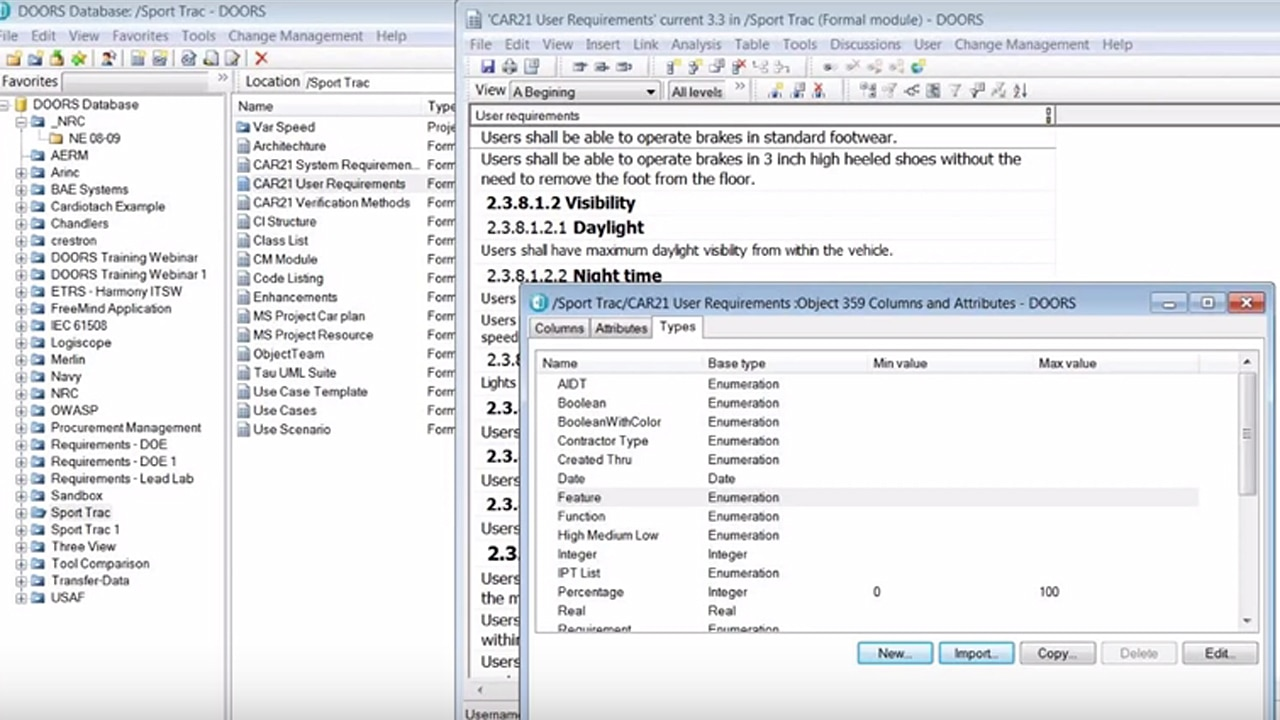
\includegraphics[scale=0.4]{images/interface_doors}
 \caption{Interface utilisateur Rational DOORS}
\end{figure}

Grâce à sa propre base de données intégrée, Rational DOORS met à notre disposition un large éventail de fonctions qui nous aident à capturer et gérer les exigences. Il permet de réduire les coûts de développement de 57\%, d'accélérer les ventes de 20\% et de diminuer le coût de la qualité de 69\%.

\subsection{CANoe}

CANoe est un outils de développement et de tests crée par \textbf{Vector Informatik GmbH}. C'est un logiciel complet pour le développement et analyse de réseaux ECU entier et d'ECU individuels. Il est utilisé avec succès par les équipementiers et fournisseurs depuis plus de 20 ans.

\begin{figure}[H]
 \centering
 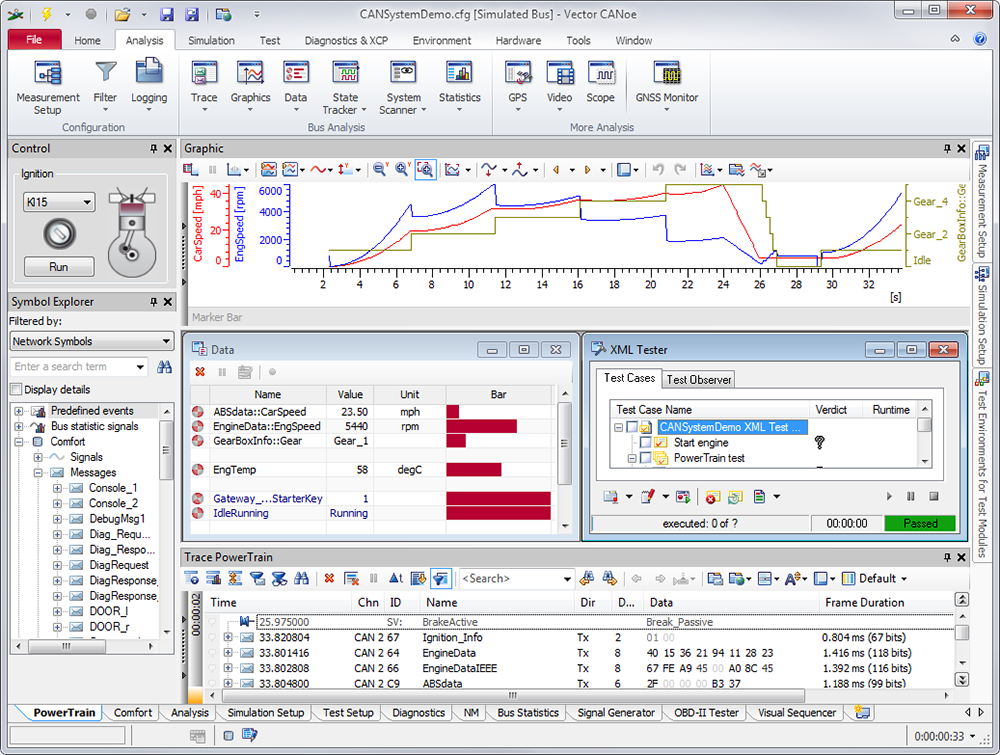
\includegraphics[scale=0.4]{images/canoe_ui}
 \caption{Interface utilisateur CANoe}
\end{figure}

\noindent CANoe supporte les systèmes de bus :
\begin{itemize}
	\item CAN (Controller Area Network)
	\item LIN (Local Interconnect Network)
	\item FlexRay
	\item Ethernet
	\item MOST (Media Oriented Systems Transport)
	\item Tout protocole basé sur le CAN.
\end{itemize} 

\medskip
\noindent CANoe contient lui même plusieurs programme : 
\begin{itemize}
	\item Avec \textbf{CANdb++ Editor} on peut créer et modifier les bases de données (*.DBC) qui contiennent des informations symbolique pour CANoe. Cela inclut les nœuds de réseau et les noms symboliques pour les messages et les signaux ainsi que les variable d'environnement.
	\item Dans \textbf{CAPL Browser} on peut créer des programmes pour la configuration des mesures et simulations.
	\item Le programme principal \textbf{CANoe} nous permet de mesurer et simuler les systèmes CAN.
	\item Dans \textbf{Panel Designer} ou \textbf{Panel Editor} on peut créer des panneaux de contrôle qui seront chargé par CANoe. Ces panneaux représentent l'interface d'entrée et sortie entre l'utilisateur et les réseaux de nœuds simulés.
	\item \textbf{CAPL Generator} est un outils qui automatise la génération des modèles de réseaux des noeuds. La génération est basée sur les bases de données CAN.
	\item \textbf{Panel Generator} est un outils qui automatise la génération des panneaux.
\end{itemize}

\begin{figure}[H]
 \centering
 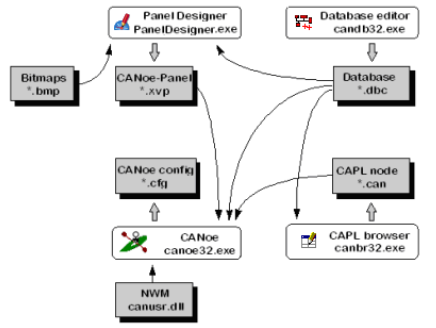
\includegraphics[scale=1]{images/global_view_canoe}
 \caption{Vue globale de CANoe}
\end{figure}

\subsection{ASAP2}

Le XCP ou bien "Protocole Universel de Mesure et de Calibration" est un réseau protocolaire qui permet de connecter les systèmes de calibration à l'ECU. Il nous donne le droit de lecture et d'écriture dans des variables et mémoire du microcontrôleur en cours d'exécution.

Une condition préalable à l'utilisation de l'XCP en tant que protocole de mesure et de calibration est l'existence d'un fichier de description ASAP2. L'outil ASAP2 est utilisé donc pour créer et vérifier ce fichier, il permet de : 

\begin{itemize}
	\item Générer automatiquement des fichiers ASAP2 en fonction des commentaires du code C.
	\item Mettre à jour l'adresse et les informations sur les types de données.
	\item Fusionner plusieurs fichiers ASAP2 dans un fichier joint.
	\item Comparer deux fichiers ASAP2 avec la documentations des résultats dans un fichier journal.
	\item Vérifier les fichiers ASAP2 pour les erreurs syntaxiques et sémantiques.
	\item Créer des dialogues et visualisations des fichier A2L.
\end{itemize}

\begin{figure}[H]
 \centering
 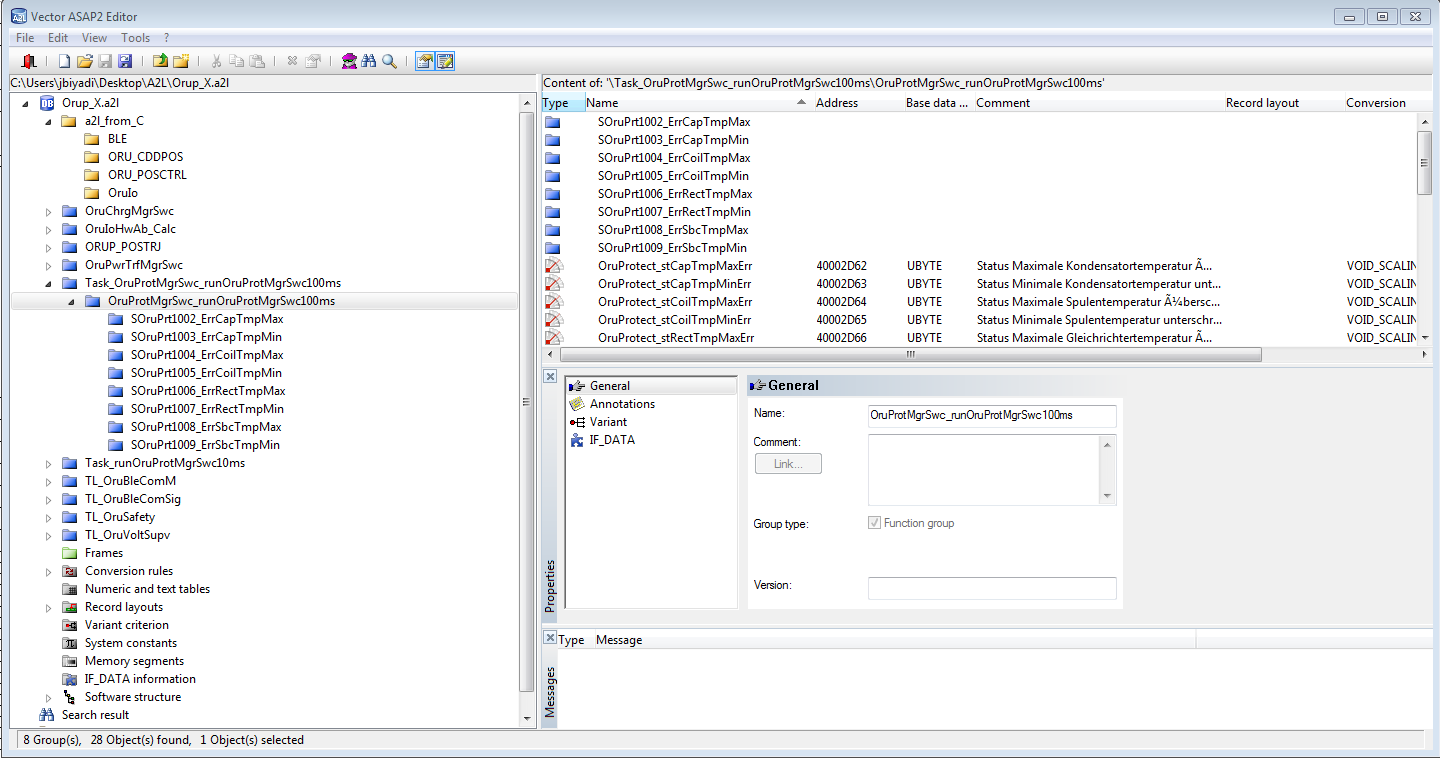
\includegraphics[scale=0.4]{images/asap_ui}
 \caption{Interface utilisateur ASAP2}
\end{figure}

\noindent L'outil ASAP2 contient lui aussi sept programmes incorporés lui permettant d'exécuter les tâches citées ci-dessus : 

\begin{itemize}
	\item ASAP2 Creator
	\item ASAP2 Updater
	\item ASAP2 Merger
	\item ASAP2 Comparer
	\item ASAP2 Checker
	\item ASAP2 Modifier
	\item ASAP2 Studio
\end{itemize}

\noindent La figure suivant représente le processus suivi pour générer un fichier ASAP2 : 

\begin{figure}[H]
 \centering
 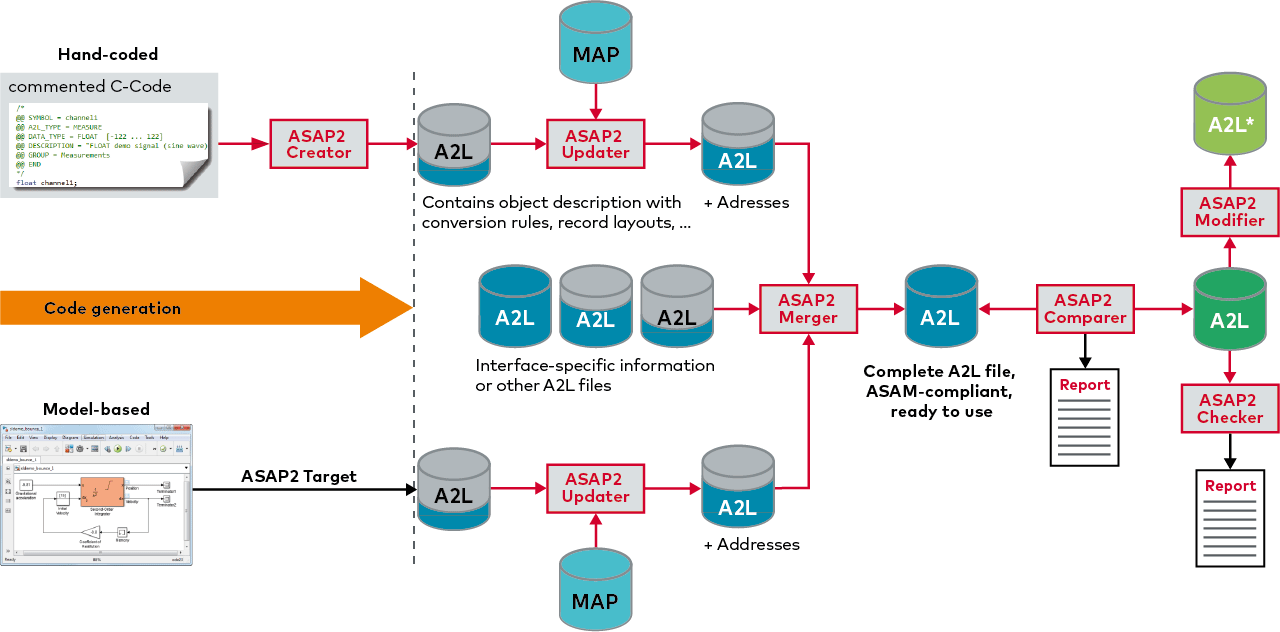
\includegraphics[scale=0.35]{images/process_a2L}
 \caption{Processus de génération A2L}
\end{figure}

Un fichier A2L peut être généré à partir de CANape à tout moment. Une autre méthode consiste à le générer automatiquement d'un code C écrit avec des commentaires spéciaux. Ce code C est analysé par A2L Creator qui est parmi les outils inclus dans ASAP2. L'algorithme cherche dans le code C des commentaires et génère une partie du A2L qui représente les paramètres de mesures et de calibration.

ASAP2 Editor lit les adresses et les typdes de données et met à jour le fichier A2L. Il permet aussi de subdiviser un fichier A2L existant en plusieurs sous-fichiers ou les joindres.




\subsection{EXAM}

Chez les constructeurs automobiles, pour la validation des systèmes électroniques embarqués, des plans de test sont élaborés. Ils couvrent un certain nombre de cas de test et s'assurent que les spécifications du besoin établies sont validées pour un système donné. Un cas de test est un chemin fonctionnel à mettre en œuvre pour atteindre un objectif de test. Un plan de test décrit également les critères d'arrêt pour la campagne, les tests effectués et surtout les tests non effectués.

Le projet décroché par ALTEN consiste à tester et valider le système AWC, pour cela nous avons eu recours à l'outil de développement graphique de test EXAM (\textbf{Ex}tended \textbf{A}utomation \textbf{M}ethod), conçu par \textbf{AUDI} et \textbf{Volkswagen}, en collaboration avec la société allemande MicroNova.

\begin{figure}[H]
 \centering
 
\includegraphics[scale=1]{images/exam_logo}
 \caption{Logo EXAM de MicroNova}
\end{figure}

EXAM définit une méthodologie complète basée sur UML pour représenter, implémenter et évaluer les cas de test. Il nous permet de modéliser graphiquement des processus de test dans des diagrammes de séquence sans connaissance avancé sur la programmation. EXAM fournit ainsi un langage uniforme pour la représentation des événements de test. Il convient à la simulation Hardware in Loop HiL, à l'automatisation des bancs de test et à l'automatisation industrielle, ainsi qu'au développement intégré et à la simulation de Software in Loop SiL.

Comme dit précédemment, EXAM a été co-développé par AUDI, Volkwagen, et MicroNova en 2006 et a été depuis établi comme un outil d'automatisation de test uniforme pour les simulateurs HiL dans tout le groupe Volkswagen.

EXAM est un outil basé sur le concept ITF (Integrated Testing Framework) : l'idée est de faciliter la collaboration entre tous les composants d'un système de test sur une plate-forme commune et intégrée. La brique EXAM, fondation de ITF, supporte toutes les tâches liées aux tests automatiques : formalisation des cas de test (diagramme séquence UML), traçabilité avec DOORS, implémentation automatique des cas de test au format Python, exécution et évaluation automatique des test sur différentes plates-formes (DSpace, MicroNova, National Instruments, Vector, ETAS, ...), ainsi que le reporting.

Vu que les scripts de test sont définis de façon uniforme avec UML, les scripts développés peuvent être exécutés et transférés automatiquement en programmes de test exécutables. La modélisation elle même est faite à l'aide de l'interface graphique, ce qui permet au développeur du test de se concentrer sur le sujet et le contenu du test sans connaître presque aucune notion de programmation.

\begin{figure}[H]
 \centering
 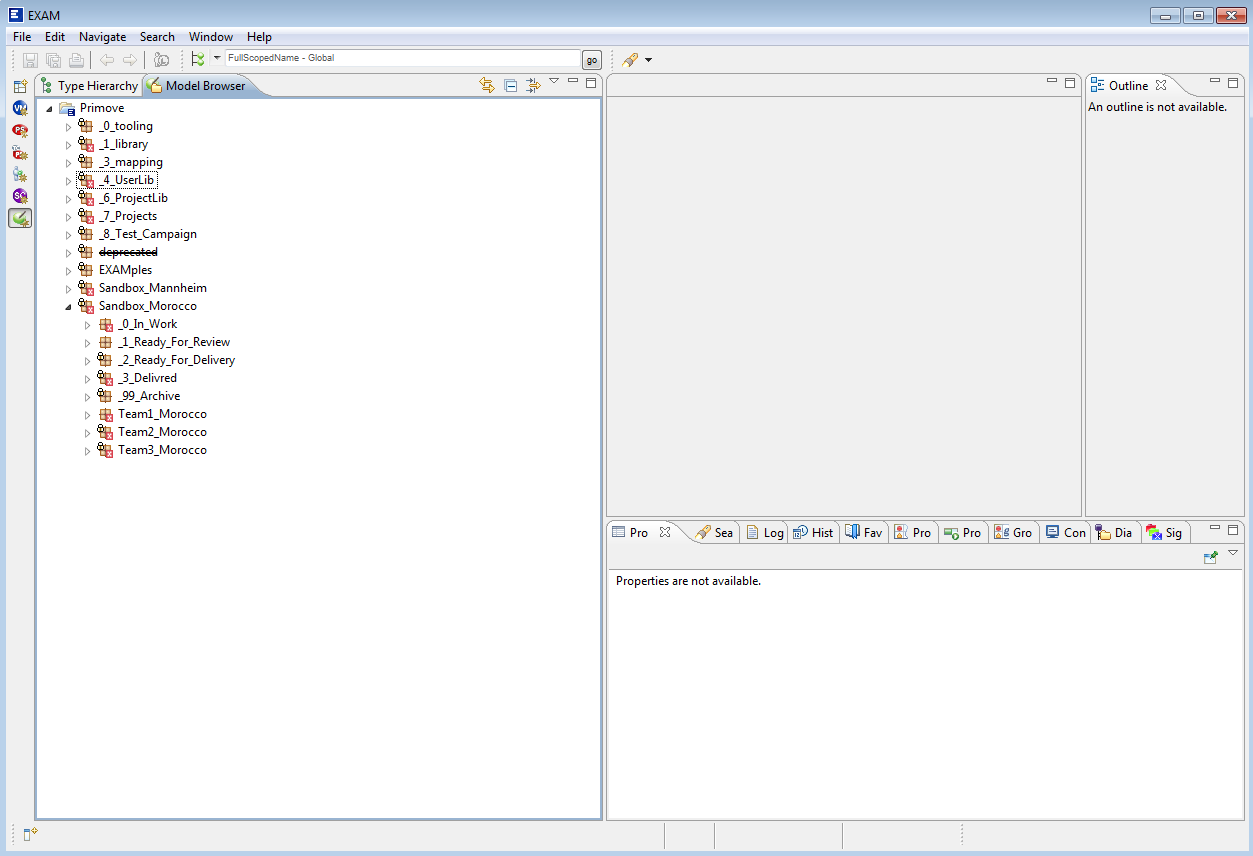
\includegraphics[scale=0.45]{images/exam_ui}
 \caption{Interface utilisateur EXAM}
\end{figure}

EXAM est une application partagé où plusieurs utilisateurs peuvent travailler simultanément sur la même donnée qui est contenu dans une base de donnée centrale. Les modifications apportées à cette donnée sont synchronisées de façon automatique. Les utilisateurs sont notifiés quand il détecte du changement dans un modèle et le recharge automatiquement.

EXAM utilise un générateur de code incrémentiel pour générer un script Python exécutable qui est utilisé pour l'exécution du test.

En plus de pouvoir modéliser les scripts de test à l'aide de l'interface graphique, EXAM nous permet de créer des scripts directement en Python. Ceci est utile lors des créations des fonctions et procédures pour faciliter le développement actuel des scripts de test.

\begin{figure}[H]
 \centering
 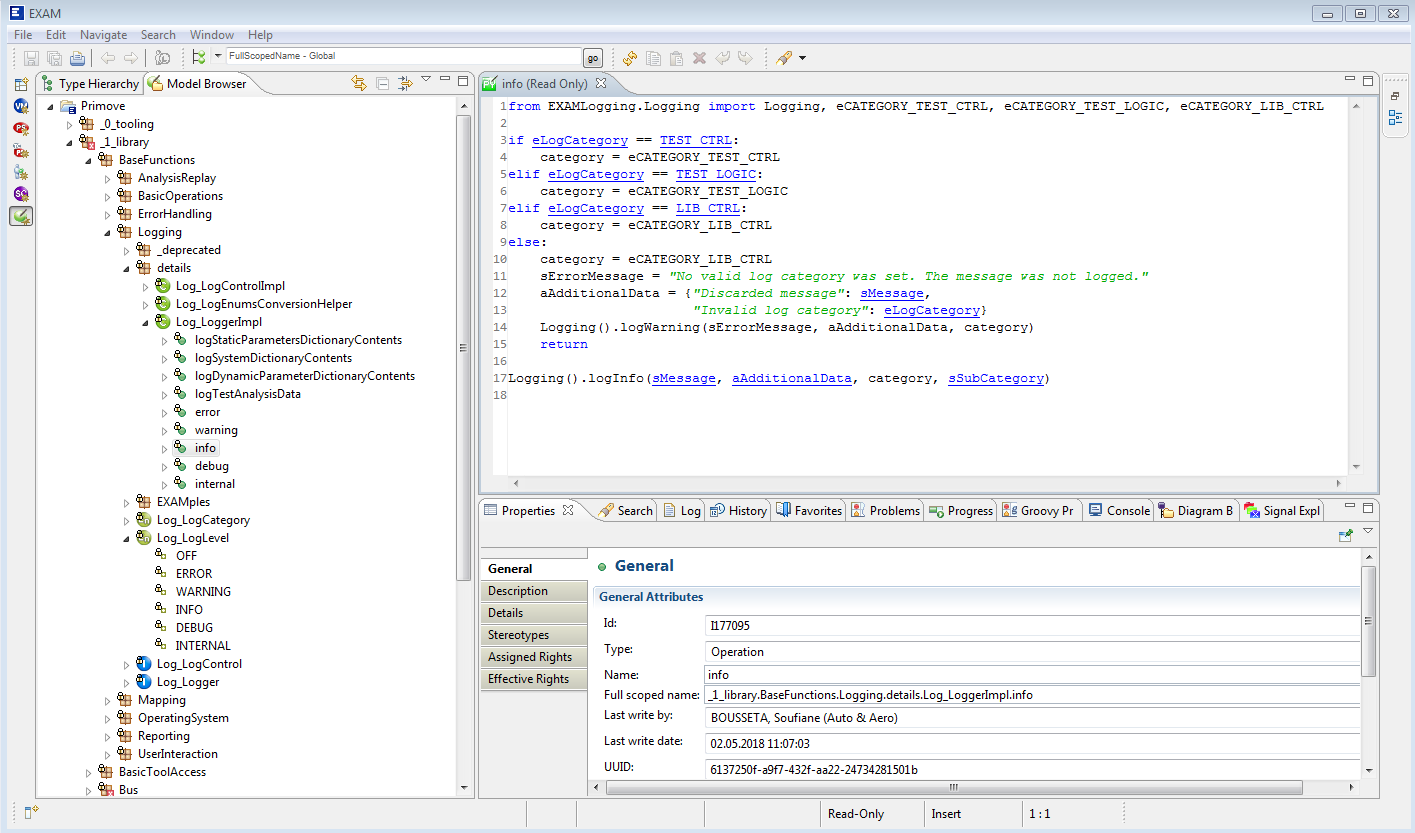
\includegraphics[scale=0.4]{images/exam_python}
 \caption{Création de script en Python avec EXAM}
\end{figure}

\subsubsection{Processus de test EXAM}

Le processus de test avec EXAM constitue seulement une partie d'un plus grand processus. Les rôles dans ce processus ne doivent pas nécessairement être remplis par une personne respectivement. Dans des petits projets, une seule personne peut jouer tous les rôles, mais dans notre cas les rôles sont affectés à chaque membre de l'équipe.

\begin{figure}[H]
 \centering
 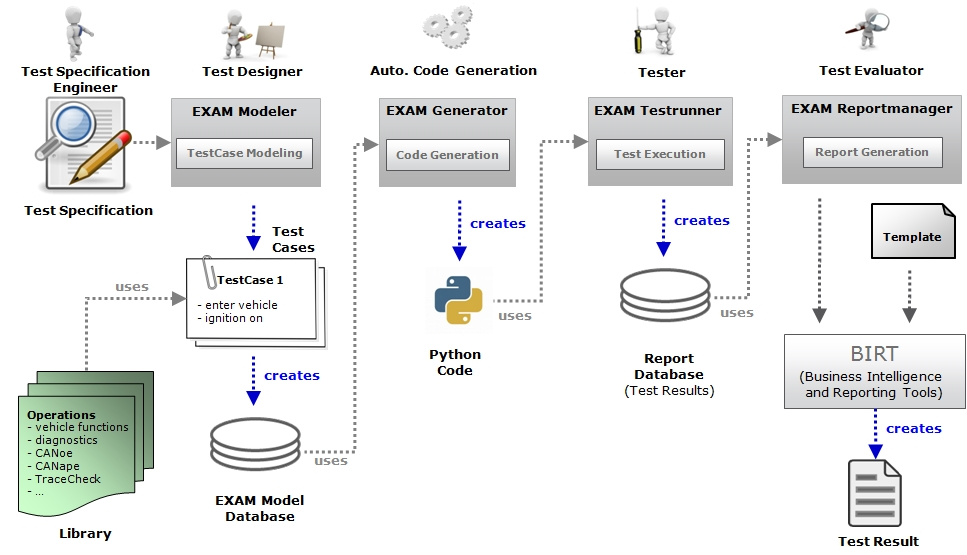
\includegraphics[scale=0.6]{images/process_exam}
 \caption{Processus de test EXAM}
\end{figure}

Le Test Manager est le rôle qui assure le suivi global du processus. Il est responsable de la planification du projet et supervise son exécution. Il définit également quelle fonction ou quelle exigence doit être testée. Cette information va être passé à l'ingénieur de test qui va développer la spécification à l'aide de Rational DOORS.

Le Designer de Test reçoit la spécification de chez l'ingénieur de test et les instructions du Test Manager. Avec ces informations il peut modéliser des tests à l'aide d'EXAM.

Le générateur d'EXAM génère automatiquement le code Python depuis le modèle crée dès l'instant où il est enregistré dans la base de donnée.

Enfin, le Testeur commence l'exécution du test sur le simulateur HiL et EXAM génère un rapport qui est sauvegardé dans la base de donnée.

